%%%%%%%%%%%%%%%%%% Część II %%%%%%%%%%%%%%%%%

\section{Rekurencyjne sieci neuronowe}

\subsection{ Kodowanie sieci neuronowych o dowolnej topologii}

\begin{itemize}
\item \textbf{
Napisz w dowolnym języku/narzędziu sparametryzowany generator warstwowych-sieci-feed-forward albo każdy-z-każdym dla f0 lub f1.}	

\begin{lstlisting}[language=python]
from random import random
import sys
'''
Simple NN generator 
Given number of neurons in each layer it generates feed-forward network in f1 notation, with random weights.
First layer is input layer: number of neurons in the first layer is equal to number of inputs of the network.
'''
def generate(neuron_type, layers):        
    print"""org:
name: Anonymous framstick
genotype:~"""
    genotype = "X"
    inputs_no = 0  
    for layer, layer_size in enumerate(layers):
        if(layer > 0):
            inputs_no = layers[layer - 1]
        first_input = 1
        for neuron in range(layer_size):
            genotype += "[%s" % (neuron_type, )
            for input_neuron in range(first_input, first_input + inputs_no):
                weight = random()
                genotype += ", %d:%f" % (-input_neuron, weight)
            genotype += "]"
            first_input +=  1
    print genotype
    print "~\n"
            

if __name__ == '__main__':
    if sys.argv[1] == '-h' or sys.argv[1] == '--help':
        print """
        Simple NN generator 
        Given number of neurons in each layer it generates
        feed-forward network in f1 notation, with random weights.
        
        usage:
            nn_generator.py N a b c
        where:
            N - number of genotypes to generate
            a - number of neurons in first layer
            b - number of neurons in second layer
            c - ...
         example:
            nn_generator.py 5 3 4 1
         will generate 5 genotypes, each with neural network of architecture 3-4-3."""
    else:
        N = int(sys.argv[1])
        layers = [int(c) for c in sys.argv[2:]]
        neuron_type = "Nu"
        for i in range(0,N):
            generate(neuron_type, layers)
\end{lstlisting}

\end{itemize}

\subsection{ Optymalizacja wag i topologii }

\begin{enumerate}
\item \textbf{Mutacja.}
	\begin{itemize}
		\item Ustaw parametry mutacji (Experiment->Genetics) w f0 i f1 tak, żeby dotyczyły tylko dodawania/usuwania neuronów i dodawania/usuwania połączeń. Ustaw "Neurons to add" na jeden rodzaj neuronu – Nu.
		\item Stwórz kilkanaście razy sekwencję 200 mutantów zaczynając od sieci z jednym neuronem. Co można powiedzieć o tych sekwencjach? Pomocniczo zrób wykresy liczby neuronów i połączeń neuronowych w funkcji n. 
W konsoli:
		\begin{verbatim}
		//make mutant sequence.
//ensure there is one genotype in the gene pool! 
var n,ile=200;
GenePools.group=0; //select first group
for(n=1;n<=ile;n++)
{
   GenePools.genotype=n-1; //select n-th genotype as ancestor
   GenePools.mutateSelected();
   Genotype.name="mutant "+n; //set its name to consecutive number
   GenePools.copySelected(0);
   //Simulator.print(""+n+" "+Genotype.nnsiz);
}
		\end{verbatim}

Na rysunkach \ref{fig:mutations-neurons} oraz \ref{fig:mutations-connections} pokazano odpowiednio ilość neuronów i ilość połączeń między nimi w funkcji ilość mutacji. Widać na nich, że w trakcie mutacji neurony i połączenia między nimi są zarówno dodawane jak i odejmowane, sama mutacja bez presji selekcyjnej nie prowadzi w żadnym kierunku.
		
	\begin{figure}[h]
	\centering
	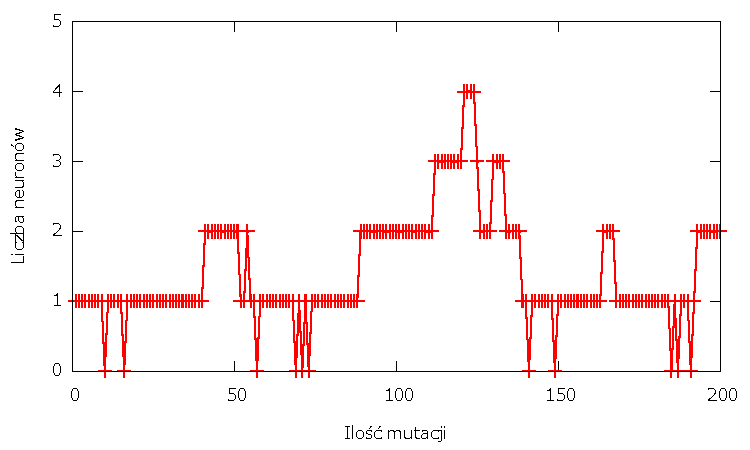
\includegraphics[width=0.8\textwidth]{dane/part2/zad2/neurons}
	\caption{Ilości neuronów w funkcji ilości mutacji.\label{fig:mutations-neurons}}
	\end{figure}
	
		\begin{figure}[h]
	\centering
	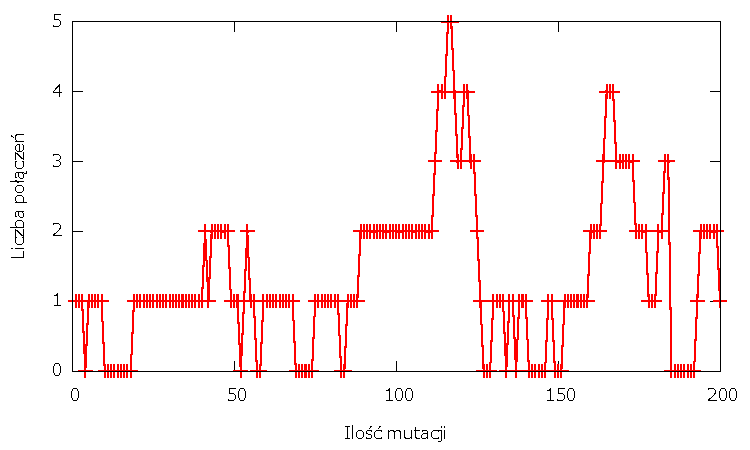
\includegraphics[width=0.8\textwidth]{dane/part2/zad2/connections}
	\caption{Ilości połączeń między neuronami w funkcji ilości mutacji.\label{fig:mutations-connections}}
	\end{figure}
		
	\end{itemize}
\item \textbf{Krzyżowanie}
	\begin{itemize}
		\item Wybierz jedną z reprezentacji: f0 lub f1.
		\item Stwórz dwie sieci neuronowe o tej samej topologii, różniące się tylko wagami.
		\item Dokonaj ich krzyżowania. Czy rezultat spełnia postulaty dobrego krzyżowania podane w poprzednim ćwiczeniu? 
		\\W konsoli:
				\begin{verbatim}
//cross over two neural networks.
//ensure there are two genotypes in the gene pool! 
GenePools.group=0; //select first group
GenePools.genotype=0; //select first genotype
GenePools.crossoverSelected(1); //cross over with the second genotype
Genotype.name="child"; //set descendant's name
GenePools.copySelected(0);
}
		\end{verbatim}
		\item Powtórz tę operację. Czy krzyżowanie jest deterministyczne?
		\item Powtórz to zadanie (krzyżowanie) dla pary sieci neuronowych o bardzo różnych topologiach.
	\end{itemize}
\end{enumerate}